\documentclass[12pt,a4paper]{article}

% ====================
% Chinese on Overleaf (XeLaTeX)
% ====================
\usepackage{fontspec}
\usepackage{xeCJK}
\setmainfont{Times New Roman}
\setCJKmainfont{TW-Kai}

% ====================
% Layout / spacing
% ====================
\usepackage{geometry}
\geometry{margin=2.2cm}
\usepackage{setspace}
\singlespacing 
\setlength{\parindent}{1.5em}
\setlength{\parskip}{2pt}

% ====================
% Figures
% ====================
\usepackage{graphicx}
\usepackage{float} 

% ====================
% Math / symbols
% ====================
\usepackage{amsmath,amssymb}

% ====================
% Lists
% ====================
\usepackage{enumitem}
\setlist[itemize]{leftmargin=2em, itemsep=1pt, topsep=2pt, parsep=0pt, partopsep=0pt}
\setlist[enumerate]{leftmargin=2em, itemsep=1pt, topsep=2pt, parsep=0pt, partopsep=0pt}


% ====================
% Links
% ====================
\usepackage[numbers,sort&compress]{natbib}
\usepackage[hidelinks]{hyperref}

% ====================
% Section titles
% ====================
\usepackage{titlesec}
\titleformat{\section}{\large\bfseries}{\thesection.}{0.5em}{}
\titleformat{\subsection}{\normalsize\bfseries}{\thesubsection}{0.5em}{}
\titleformat{\subsubsection}{\normalsize\bfseries}{\thesubsubsection}{0.5em}{}

% ====================
% Title block helpers
% ====================
\newcommand{\DocTitle}[1]{\begin{center}\Large\bfseries #1\end{center}}
\newcommand{\RuleLine}{\vspace{0.4em}\hrule\vspace{0.4em}}


\usepackage{xcolor}
\newif\ifsubmit
%% Switch to submittrue to hide all todo's and comments.
\submitfalse
%\submittrue
\ifsubmit
    \newcommand{\graceY}[1]{#1}
    \newcommand{\kelly}[1]{#1}
    \newcommand{\sangjung}[1]{#1}
    \newcommand{\yishin}[1]{#1}
\else
    \newcommand{\graceY}[1]{\textbf{\textcolor{purple}{graceY: #1}}}
    \newcommand{\kelly}[1]{{\textcolor{orange}{old: #1}}}
    \newcommand{\sangjung}[1]{{\textcolor{teal}{#1}}}
    \newcommand{\yishin}[1]{{\textcolor{teal}{#1}}}
\fi








\begin{document}
% =========================================================
% Cover / Header
% =========================================================
\DocTitle{115年度國科會大專學生研究計畫申請書}

\noindent
\textbf{計畫名稱：}
基於多層級記憶協調與角色向量建模之虛擬研究指導老師系統\\
\textbf{Project Title:}
Designing a Trajectory-Aware Virtual Research Mentorship System through Multi-Level Memory Coordination and Persona Modeling

\RuleLine



% =========================================================
% 1. Abstract
% =========================================================
\section*{一、摘要}
\addcontentsline{toc}{section}{一、摘要 (Abstract)}
在學術人才培育中，研究指導會議不僅推動研究進展，亦是培養學生表達、釐清與修正研究想法的重要互動場域。隨著大型語言模型（Large Language Models, LLMs）逐漸被引入教育與學術輔導情境，已有不少研究嘗試以虛擬系統擔任研究導師或助教。然而，現有多數基於 LLM 的虛擬助教系統仍仰賴通用指導原則或預設角色特性，難以反映研究指導中高度互動且具連續性的實務特性。

本計畫聚焦於現有虛擬研究指導系統在實務應用上的三項關鍵限制：
(一) 研究歷程之邏輯銜接不順：即系統未能有效納入跨會議的研究演進脈絡，包含研究方向的轉折與反覆修正歷程，導致對當前指導目標的理解與實際研究狀態產生落差。
(二) 角色人格漂移（persona drift）：即虛擬助教的指導風格與專業界線容易受到即時語境影響而偏移，進而產生迎合式建議，降低長期互動中回應內容的可靠性 。
(三) 互動臨場感不足：現有系統多採用通用型大型語言模型，回覆傾向標準化且高度中立，難以呈現真實學術情境中個別教授獨有的指導風格與互動習慣，導致對話過程流於機械化，缺乏臨場感。

為回應上述挑戰，本研究提出一套整合多層級記憶協調與角色向量建模之虛擬研究指導對話系統。系統透過分層記憶架構整合即時對話脈絡、近期研究活動摘要與長期研究歷程紀錄，以維持跨會議互動的邏輯一致性；同時，導入即時監控的推理階段介入機制，以在必要時對模型輸出進行干預，將真實研究指導會議中的互動模式融入角色向量之建模，以維持穩定且具臨場感的指導行為。最後，本研究將建立對應長期互動情境的評估方法，針對研究歷程連貫性、指導角色穩定性與互動臨場感等關鍵面向進行系統性驗證，作為評估虛擬研究指導系統是否能貼近真實 mentor--mentee 配對關係的重要依據。

本研究預期發展一套可實作且可評估的虛擬研究指導系統設計架構，使人工智慧能在跨會議、跨研究階段的互動中，維持對研究歷程與指導角色的穩定理解。研究成果可作為未來研究指導與高等教育人機協作系統的設計基礎，使其更適用於實際研究訓練情境，並為相關系統的設計與評估提供具體經驗。此外，透過對長期研究指導會議狀態與互動歷程的分析，本研究亦有助於促進研究指導經驗的系統化整理與分享。

% =========================================================
% 2. Motivation & Research Questions
% =========================================================
\section*{二、研究動機與研究問題}
\addcontentsline{toc}{section}{二、研究動機與研究問題}

\subsection*{(一) 研究動機}
本計畫聚焦於學術專題指導中「高度非線性議題演進」與「長週期進度追蹤」之複雜情境。在高等教育互動中，指導品質的核心取決於「教授人設穩定性（Persona Stability）」及其背後的學術權威立場。專題研究通常橫跨數月，涉及多次會議中研究假設之更迭、方法論之修正及實驗路徑之調整，對虛擬指導系統的記憶能力與角色穩定性提出嚴峻挑戰。

在記憶層面，現有大型語言模型（LLM）的記憶機制多侷限於片段式資訊存取，缺乏能表徵「研究過程決策因果依賴鏈」的結構化載體，難以在動態變化的研究決策中提供長程邏輯一貫的專業指導。MemoryBank 與 MemGPT 雖提供了長效存儲機制 \citep{a2305_10250v3_memorybank, a2310_08560v2_memgpt}，但面對高度邏輯嵌套的學術情境，仍難以達到圖式記憶（Graph-based Memory）在結構一致性與邏輯關係追蹤上的效果 \citep{a2602_05665v1_graphagentmemory}。

在角色一致性層面，有效的學術輔導要求虛擬導師維持批判性、方法論的嚴謹、對證據敏感並避免盲目迎合；系統若能忠實再現真實指導者的行為特徵，將有助於建立長期互動中的專業信任感。然而，LLM 的行為表現往往隨對話歷史而偏差，損害指導的可信度。近年 Persona Vectors 研究顯示，模型的人格特質可在激活空間（Activation Space）中以近似線性的方向被監測 \citep{a2507_21509v3_personavectors}；表徵工程（Representation Engineering）與推理時干預（Inference-time Steering）的進展則進一步證實，透過激活值加法（Activation Addition）等手段，可在不重新訓練的前提下，有效干預並校正模型的行為方向 \citep{turner-etal-2023-activation-addition, wehner-etal-2025-representation-engineering}。

基於上述背景，本研究的核心動機在於結合「記憶結構的穩固化」與「生成行為的即時校正」：透過「圖式長期記憶」維持跨會議的研究邏輯鏈，確保建議內容的事實一致性；同時利用「人設向量」於推理時進行即時監控與控制，確保指導風格的一致性。本計畫旨在建立一個在長週期專題輔導中更具邏輯記憶、可量測且指導風格穩定的虛擬教授系統。

\subsection*{(二) 研究問題}
本研究將以「長程一致性」為主軸，提出以下可驗證之研究問題（Research Questions, RQs）：

\begin{itemize}

  \item \textbf{RQ1（研究脈絡一致性）}：相較於僅使用文字記憶（非結構化摘要或片段檢索），以 Dependency Graph 建模之長期記憶是否能顯著降低跨會議對話中的研究邏輯斷裂與矛盾（例如目標變動、方法自相矛盾、TODO 遺失），並提升指導建議的可追溯性（traceability）與可檢核性？
  \item \textbf{RQ2（人設穩定性與漂移抑制）}：透過人設向量（Persona Vector）進行推理時干預，是否能在長程對話中維持指導教授互動策略的一致性，並以量化方式降低 persona drift 的發生程度？
  \item \textbf{RQ3（教育指導品質的外部效度）}：在真人盲測情境下，具備圖式長期記憶與人設向量監控之系統，是否能在指導品質量表（如 MCA-21）與 AI 導師評測框架中獲得顯著較佳的評分，並展現可部署的可靠性提升？
\end{itemize}

%=========================================================
% 3. Related Work / Literature Review
% =========================================================
\section*{三、文獻回顧與探討}
\addcontentsline{toc}{section}{三、文獻回顧與探討}

本章節將回顧三個相關研究領域的重要進展：(i) LLM 教育導師之能力與評測、(ii) 長程對話的記憶與跨會議一致性建模、(iii) 人設（persona）表徵與推理時控制（inference-time steering/representation engineering），並說明本研究如何建構於既有成果之上，進一步拓展其理論與方法。

\subsection*{(一) LLM 教育導師：任務形式、能力評測與「長期指導一致性」缺口}
教育導師類系統近年逐漸由「單輪答題」走向「多輪教學互動」與「情境式指導」。BEA 2023 shared task 已將 AI 教師回應生成視為可進行系統化評測的教育對話任務，凸顯教學回應需要兼顧\emph{教學策略、對話連貫與錯誤處理}等要素 \citep{tack-etal-2023-bea}。然而，多數評測仍偏重於短期互動品質，較少直接處理「跨多次會議」的學術指導一致性問題。

為補足評測面向上的缺失，近期開始出現以「導師能力」為核心的系統化評估框架與基準集。例如 Maurya et al.~\citep{maurya-etal-2025-unifying} 提出針對 LLM 導師教學能力的評測架構（taxonomy），將教學能力拆解為多維度（如回饋品質、引導策略、錯誤診斷、適應性等），為本研究後續「指導品質」指標設計提供參考。進一步地，針對 LLM 導師的 benchmark 亦逐漸成形（例如以教學任務、題型或互動策略為主軸），用以量化不同模型與系統設計在教育場景的行為差異 \citep{a2510_02663v1_tutorbench,a2601_21375v1_teachbench}。

另外，除了「回答品質」的評測，亦有研究直接聚焦在「導師—學生」互動的對話策略如何啟動研究討論。例如，Faff~\citep{faff2024prfai_ssrn4999390} 以研究導師主導的提問與回饋策略設計（並結合 PRF-AI 混合工具）探討如何引導學生逐步收斂研究題目與方法路徑。此一脈絡對本研究的啟示在於：虛擬教授不僅需能回答問題，更需在跨會議中持續以「導師式對話策略」推進研究決策與任務分解，才能對應專題指導的真實需求。

此外，人機互動（HCI）研究亦指出學習者與 AI 導師互動時，對「角色穩定性」與「信任」具有高度敏感性：同一系統若在不同回合呈現不一致的指導風格或目標變動，會直接削弱學習者對系統的信賴感與持續使用意願 \citep{tutorup_chi2025,mentigo_chi2025}。綜合而言，現有文獻已提供\emph{教學能力拆解}與\emph{導師基準評測}，但對「長期指導一致性」尚缺少可操作的系統設計與可量測的控制機制；本研究即以此缺口為核心切入點。

\subsection*{(二) 長期對話記憶：從記憶模組到協調策略}
要維持長期一致性，第一個瓶頸在於「記憶」：LLM 若僅依賴上下文視窗或片段摘要，容易在跨會議時遺失研究決策、TODO 與依賴關係。對此，近年多篇工作提出將外部記憶納入 LLM 系統的架構，強調「\emph{短期／長期記憶分工}」與「\emph{檢索＋更新}」迴路。MemoryBank 以長期記憶增強個人化對話，強調對話歷程的持續累積與檢索，以改善後續互動的一致性 \citep{a2305_10250v3_memorybank}。MemGPT 則將 LLM 視為「作業系統式」代理，透過記憶層級與管理策略，在有限上下文下維持長期任務表現 \citep{a2310_08560v2_memgpt}。
同樣地，在高風險領域的個人化助理場景中，亦有研究提出以\emph{短期記憶}（近期對話狀態）與\emph{長期記憶}（穩定使用者偏好／背景）協同運作的設計，並討論兩者在更新頻率、衝突解決與安全性上的權衡 \citep{zhang-etal-2024-llm-based}。近期亦有針對記憶系統的評測與分析工作，指出記憶寫入／淘汰策略、檢索噪聲與錯誤累積，會顯著影響長程對話品質與可靠性 \citep{a2402_17753v1_locomomemoryeval,a2505_16067v2_memorymanagementimpacts}，並提出更系統化的「記憶層管理」觀點與工具化實作 \citep{a2504_19413v1_mem0,a2507_07957v1_mirix}。

然而，上述記憶系統多以「\emph{文本片段}」作為儲存單位，對「研究專題」這類高度依賴\emph{方法假設、實驗依賴與決策鏈}的任務而言，僅靠片段記憶仍可能出現「檢索到資訊卻無法維持推理一致」的情形。本研究因此主張：記憶不只要能保存與取回，還必須可結構化地表徵研究依賴關係，才能在跨會議推理中提供可檢核的一致性支撐。

\subsection*{(三) 會議導向的摘要與組織記憶：從對話摘要到議程／決策導向}
本研究場景（專題會議）本質上屬於多輪、多人、目標驅動的對話序列，與「會議摘要／會議記憶」研究高度相關。早期工作已探討如何從多說話者對話中萃取可讀摘要，並處理冗餘、話輪交錯與資訊重要性判定等問題 \citep{zechner2001concise_dialogue_summaries,wang-cardie-2011-summarizing}。近期工作進一步將\emph{議程（agenda）}、\emph{決策點}與\emph{行動項（action items）}視為會議摘要的關鍵結構，強化「可追蹤的會議脈絡」而非僅生成流暢文字 \citep{liu2025agendaaware_meetingsum,laskar-etal-2023-building}。這些研究共同指出：會議資訊的價值在於其可執行性與可追溯性，特別是「決策理由」與「後續行動」對長程任務影響最大。

對「專題指導一致性」而言，會議摘要若只生成自然語言段落，仍難以穩定支援跨會議推理：同一 TODO 的前置條件、方法修改的理由、實驗失敗的原因與替代方案等，往往需要以結構化關係被保存，才能避免後續指導在不同會議間互相矛盾。故本研究以「Dependency Graph」作為長期記憶載體，將會議輸入由摘要提升為\emph{可運算、可檢核}的研究依賴表示。

\subsection*{(四) 圖式／結構化長期記憶：以 Dependency Graph 支撐跨會議推理}
圖式記憶近年在 LLM 代理領域快速發展，其核心概念是讓系統以節點／邊表示「事實、關係、因果、任務分解」並支援精準檢索與一致性檢查。GraphAgentMemory 強調以圖結構組織代理的經驗與知識，可提升多步推理與長期任務的穩健度 \citep{a2602_05665v1_graphagentmemory}。此類方法與傳統「僅以向量檢索記憶片段」相比，關鍵優勢在於：圖能顯式表示依賴鏈與衝突檢查規則，使跨會議的一致性可以被系統性地檢測（例如：若節點 A 依賴 B，但 B 尚未完成，則禁止輸出與 A 完成相矛盾的結論），從而降低跨會議推理中產生邏輯矛盾的可能性。

本研究採「多層次記憶協調」：Working/Short-term Memory 著重即時對話與近程 TODO；Long-term Memory 以 Dependency Graph 保存研究脈絡（目標、假設、方法、實驗、結果、決策、TODO）及其依賴關係。這樣的設計使「一致性」不再僅靠模型自發保持，而是由外部可檢核結構提供約束與提示，形成可落地的系統化可靠性路徑 \citep{a2310_08560v2_memgpt,a2602_05665v1_graphagentmemory}。

\subsection*{(五) Persona Drift 與可控人設：從角色設計到表徵監控}
第二個長跨度失效在於 persona drift：在長期互動中，模型可能受使用者回覆影響而偏移為迎合式、逢迎式回應，或失去學術嚴謹的指導風格。教育對話研究早已指出「角色」與「回應意圖」會顯著影響學習成效與互動品質；例如對話意圖與角色策略的建模，被用於使系統在不同教學階段產生適切回應 \citep{petukhova-kochmar-2025-intent,tao-etal-2024-rolecraft}。然而，傳統角色設計多透過 prompt 或資料蒐集維持，較難在長期對話中提供\emph{可量測、可干預}的穩定性保證。

Persona Vectors 的研究提出：人設特質可在模型內部表徵空間中以方向向量近似，並可用於監測與引導生成行為，提供「\emph{以表徵為介面}」的控制途徑 \citep{a2507_21509v3_personavectors}。此一觀點對本研究至關重要：我們不僅要「定義教授人設」，更要能量化當前生成是否仍對齊教授式指導特質，並在偏移時採取即時校正。

\subsection*{(六) 推理時干預與表徵工程：以 Residual Stream 操控提升可靠性}
在不進行高成本 retraining 的前提下，「推理時干預」提供一條輕量、可部署的可靠性策略。Activation Engineering 類方法展示可透過在激活空間加入特定方向來 steer 模型行為，並以較低代價達成顯著控制效果 \citep{turner-etal-2023-activation-addition}。Representation Engineering（RepE）綜述更系統地整理「辨識表徵—操作化—控制」的流程與挑戰，指出表徵操控在多概念管理、可靠性與效能保持方面仍需嚴謹設計 \citep{wehner-etal-2025-representation-engineering}。

在更廣義的「代理式（agentic）」系統設計上，ReAct 以「推理—行動」交替的格式化軌跡，證明語言模型可在思考過程中適時呼叫工具或外部知識，以提升任務完成率與可解釋性 \citep{Yao2023ReAct}；Reflexion 進一步引入自我反思與經驗記錄，讓代理能在失敗後以自然語言回饋形成更穩定的行為策略 \citep{Shinn2023Reflexion}。此外，Generative Agents 顯示多代理的日常行為可由記憶、反思與規劃（planning）驅動而產生可持續互動 \citep{Park2023Generative}。上述研究為本計畫的系統化設計提供補強：除記憶與表徵操控外，我們亦可在虛擬教授的推理流程中納入「反思—修正」迴路與可追溯的行動記錄，使跨會議指導更具可檢核性與可重現性。
綜合上述表徵工程與代理式系統的進展，本計畫據此設計「即時人設向量監控（以內積投影量測）」與「自適應 steering（動態調 $\alpha$）」：以內積分數作為一致性量測，再於中後層殘差流注入教授人設向量進行校正，使 persona drift 可被監測並被即時抑制。

\subsection*{(七) 小結：研究定位與貢獻缺口}
綜合上述，現有文獻在各面向均已累積重要基礎：教育導師評測框架與 benchmark \citep{maurya-etal-2025-unifying,a2510_02663v1_tutorbench,a2601_21375v1_teachbench}、長期記憶系統與管理策略 \citep{a2305_10250v3_memorybank,a2310_08560v2_memgpt,a2504_19413v1_mem0}、會議摘要與決策導向表示 \citep{liu2025agendaaware_meetingsum,laskar-etal-2023-building}，以及 persona 表徵與推理時控制 \citep{a2507_21509v3_personavectors,turner-etal-2023-activation-addition,wehner-etal-2025-representation-engineering}。
但這些脈絡尚未被整合，尚缺少一個針對「跨會議學術指導」的整合式系統：同時以圖式長期記憶確保研究脈絡一致，並以表徵層的人設監控＋推理時干預來抑制 persona drift。本研究即以此整合缺口為目標，提出可實作的架構與可量測的評估設計，作為高可靠性教育代理之方法論參考。
% =========================================================
% 4. Methods & Steps
% =========================================================
\section*{四、研究方法及步驟}
\addcontentsline{toc}{section}{四、研究方法及步驟}

\graceY{本計畫分為兩個主要階段。\textbf{第一階段為模擬教授系統的建置與模型發展}，主要工作包括研究指導會議資料的蒐集、資料前處理與結構化流程的建立，以及模型架構設計與建模實作。考量研究倫理審查與個資保護規範，計畫初期將以申請人本人與指導教授的研究會議錄音作為訓練與方法驗證基礎。雙方已累積半年以上的會議紀錄，具備足夠樣本量支援前期模型測試與機制調整。本階段核心目標在於建構支援長期研究歷程表示的記憶機制，以及維持指導角色一致性的對話架構。}

\graceY{\textbf{第二階段為系統的技術效能評估與使用者實證研究}。技術層面將透過與現有最先進方法（state-of-the-art, SOTA）比較，評估生成對話在研究歷程連貫性、角色穩定性與互動一致性等面向的表現，並檢驗其與真實研究指導情境的相似程度。使用者層面則透過控制實驗與半結構式訪談，分析使用者對互動臨場感與角色真實性的主觀感受，以及系統於會議預演（rehearsal）情境中的實際效益與可能限制。以下為兩階段的研究方法:}


%本研究採「系統建構 + 壓力測試 + 真人盲測」的混合方法，目標是同時驗證：(i) 跨會議研究脈絡一致性是否提升，(ii) 教授式人設是否能被\emph{量測}與\emph{即時校正}，並在教學與指導品質上獲得顯著改善 \citep{maurya-etal-2025-unifying,tack-etal-2023-bea}。

\subsection*{(一) 階段一：系統架構建置與對話模型建立}

\subsubsection*{1. 虛擬教授代理人之多層次記憶協調建置（Working / Short-term / Long-term））} 

\paragraph*{Working Memory（即時對話工作記憶）}
Working Memory 定義為單次互動中可直接提供模型的上下文訊息，包含：當前會議的即時對話逐字稿，以及系統側即時產生的「狀態摘要」（例如本輪目標、當前假設、需要澄清之點）。此層主要用於確保回覆連貫與避免短期對話遺漏，並為後續 Short-term / Long-term 的寫入提供結構化事件（event）單位 \citep{a2310_08560v2_memgpt}。

\paragraph*{Short-term Memory（近三次會議進度與 TODO 記憶）}
Short-term Memory 以「近三次會議」作為時間窗的設定，保存具可執行性的行動項（action items）、未完成 TODO、近期方法變動與實驗待辦。此層提供快速檢索與更新（append/resolve）的能力，並採用版本化（versioned）條目，記錄「提出者、提出時間、依賴前置、完成狀態」，以支援一致性檢核與責任歸屬 \citep{a2305_10250v3_memorybank,a2504_19413v1_mem0}。

\paragraph*{Long-term Memory（研究依賴圖：Dependency Graph）}
Long-term Memory 採用 Dependency Graph 表徵跨會議研究脈絡，將專題研究拆解為節點（nodes）與邊（edges）：
\begin{itemize}
  \item 節點類型：Research Goal、Hypothesis、Method/Design Choice、Experiment、Result、Decision/Rationale、TODO/Next Step。
  \item 邊類型：\texttt{depends\_on}（依賴）、\texttt{supports}（證據支持）、\texttt{contradicts}（衝突）、\texttt{refines}（細化/修正）、\texttt{blocks}（阻塞）。
\end{itemize}
每次會議輸入後，系統從對話中抽取「決策點、理由、結論、後續行動」，並以增量方式更新圖；同時維持「可追溯路徑」（從 Goal $\rightarrow$ Method $\rightarrow$ Experiment $\rightarrow$ Result $\rightarrow$ Decision），以支援跨會議一致性檢查與對齊提示 \citep{a2602_05665v1_graphagentmemory,laskar-etal-2023-building,liu2025agendaaware_meetingsum}。

\subsubsection*{4. 記憶協調策略（Update / Retrieve）}
本研究採兩段式流水線：
\begin{enumerate}
  \item \textbf{Update}：在會議過程中對話逐字稿會持續寫入 Working memory，每次對話/會議結束後，將新資訊分派寫入 Short-term 與 Long-term（圖）。對於「方法修正」或「結論翻轉」事件，必須生成 \texttt{refines} 或 \texttt{contradicts} 邊，以顯式標記變更脈絡。
  \item \textbf{Retrieve}：模型回覆前，先以使用者問題作為查詢，檢索 (i) Working 中的相關對話、(ii) Short-term 中相關 TODO/狀態、(iii) Long-term 裡 Dependency Graph 中與當前 Goal 相連的最短依賴鏈與最新決策節點，組合成「研究脈絡提示」。
\end{enumerate}

\begin{figure}[H]
  \centering
  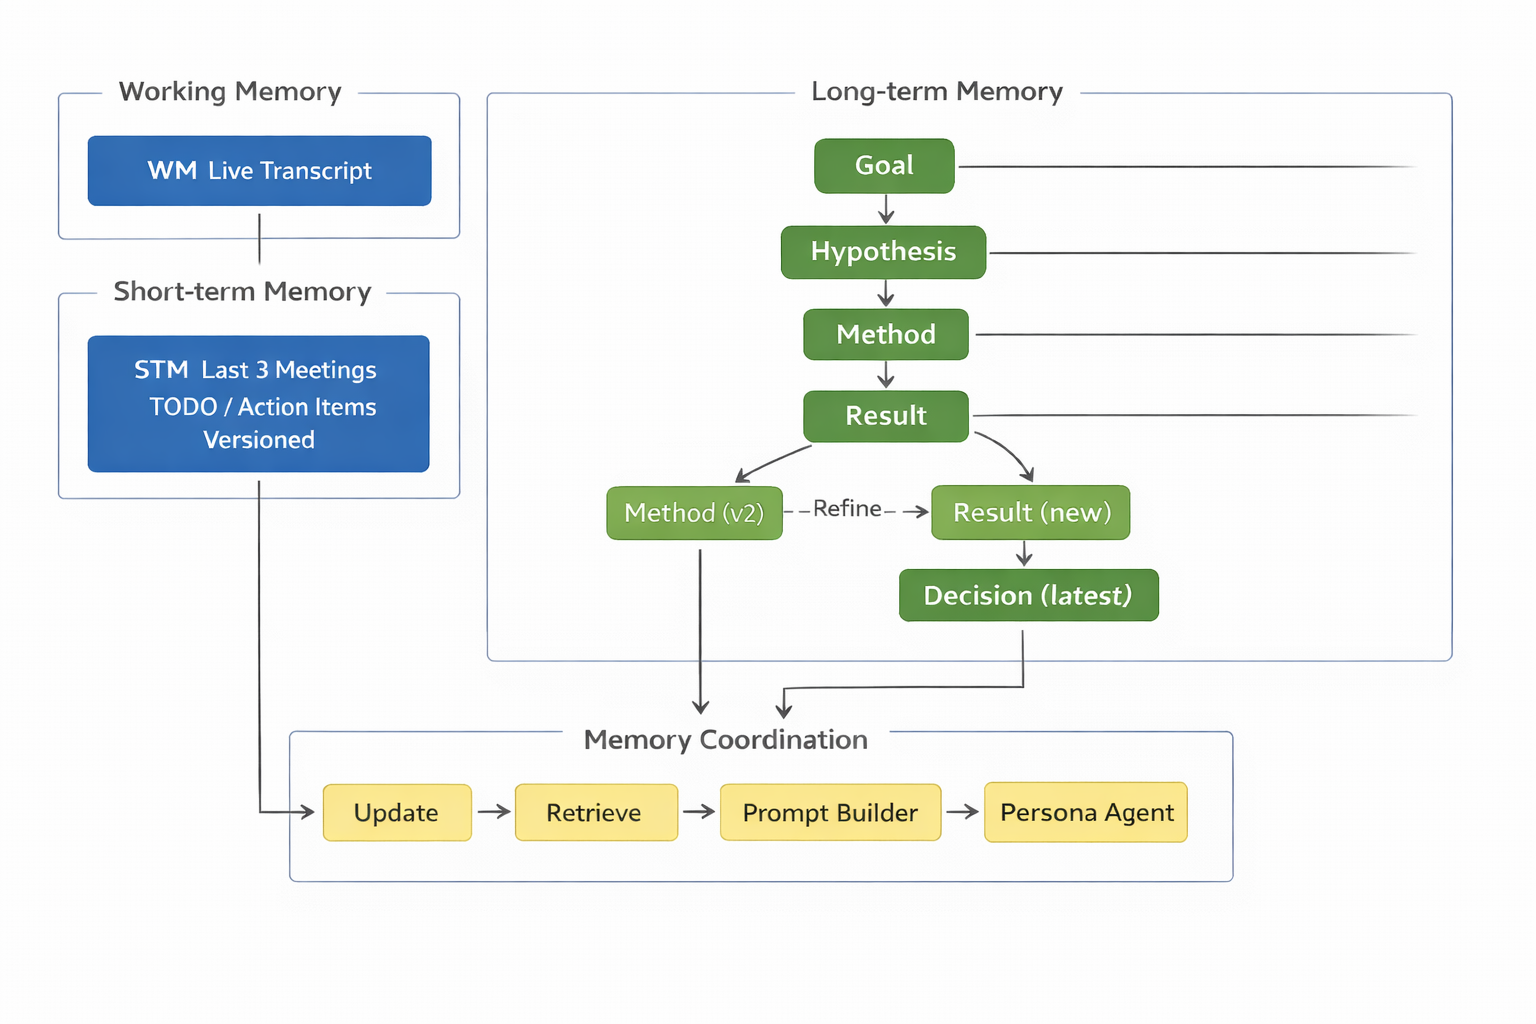
\includegraphics[width=\linewidth]{figures/memory_architecture.png}
  \caption{多層次記憶協調架構：Working/Short-term/Long-term Memory 與 Update-Retrieve 之協調流程。}
  \label{fig:memory-architecture}
\end{figure}


\subsection*{(二) 基於表徵干預之指導人設一致性監控機制（Persona Consistency Monitoring via Representation Steering）}
本研究採用 persona 表徵方向來量測「教授式導師」的人設一致性，並以推理時干預抑制 drift \citep{a2507_21509v3_personavectors}。核心作法如下：
\paragraph{(a) 自動化人設向量提取（Automated Persona Vector Extraction）}
為了獲得高保真度的 $v_{\text{professor}}$，本研究採用 Chen et al. \citep{a2507_21509v3_personavectors} 提出之自動化對比提取流程：
\begin{enumerate}
    \item \textbf{對比數據生成}：本研究自實際會議對話資料中，歸納並定義『教授式導師』之關鍵特徵描述（如學術嚴謹性、蘇格拉底式引導問答）；隨後利用大型語言模型生成 $N$ 組成對指令數據，藉由構建正、負向系統提示詞的對比，在語義空間中精準捕捉該人格特質的方向（Positive/Negative System Prompts）。
    \item \textbf{激活值採樣}：將學術問題集 $\mathcal{X}$ 輸入模型，提取模型在殘差流（Residual Stream）中的激活狀態。
    \item \textbf{向量計算}：採用均值差異法（Difference-in-Means）計算人設向量。公式如下：
    \begin{equation}
        v_{\text{professor}} = \frac{1}{|\mathcal{D}|} \sum_{x \in \mathcal{D}} \left( \mu(x)_{\text{pos}} - \mu(x)_{\text{neg}} \right)
    \end{equation}
    其中 $\mu(x)$ 代表模型生成回答時所有 token 的殘差流的平均激活值。此向量 $v_{\text{professor}}$ 即代表「學術指導人格」在激活空間中的線性方向。
\end{enumerate}
\paragraph{(b) 雙重一致性監控機制（Dual Consistency Monitoring）}
本研究建立預測性與即時性兼具的監控機制，以量化「教授式導師」的人設狀態：
\begin{itemize}
    \item \textbf{預測性監控}：在模型生成回答前，計算最後一個提示詞標記（Last Prompt Token）之激活值 $h_{\text{last}}$ 在 $v_{\text{professor}}$ 上的投影。研究證實此指標可提前預測後續生成是否偏離人設，作為預先攔截之依據 \citep{a2507_21509v3_personavectors}。
    \item \textbf{即時一致性分數}：在解碼過程中，計算每一步驟激活投影之滑動平均 $S = \text{EMA}(\langle h_l, v_{\text{professor}} \rangle)$。當 $S < \tau$ 時，視為人設偏移風險上升（如出現順從性回應傾向）。
\end{itemize}
\paragraph{(c) 推理時殘差流干預（Inference-time Steering）}
針對偵測到的人設偏移，本研究不採用重訓練模式，而是在推理時於特定層次介入殘差流，其核心更新式如下：
\begin{equation}
    h_l \leftarrow h_l + \alpha \cdot v_{\text{professor}}
\end{equation}
其中 $h_l$ 為第 $l$ 層原始激活值，$v_{\text{professor}}$ 為引導向量，$\alpha$ 為自適應干預強度係數 \citep{turner-etal-2023-activation-addition}。

\paragraph{(d) 層次選擇與自適應調整策略（Layer Selection and Adaptive Steering）}
為優化干預效率並平衡生成品質，本研究採取以下策略：
\begin{enumerate}
    \item \textbf{因果干預掃描（Causal Steering Sweep）}：透過逐層干預測試，選擇特徵表達最強且語言流暢度（Perplexity）損失最小的層次（預計為第 16--20 層）作為最終部署層 \citep{a2507_21509v3_personavectors}。
    \item \textbf{動態調整強度}：系統依據即時分數 $S$ 與閾值 $\tau$ 進行反饋調節。若 $S < \tau$，則線性調升 $\alpha$ 以強化人設立場；若一致性回歸正常，則逐步回退 $\alpha$ 以確保回覆的自然度與流暢度 \citep{wehner-etal-2025-representation-engineering}。
\end{enumerate}

\subsection*{(三) 實驗設計：自動化壓力測試與真人盲測}
\subsubsection*{1. 自動化壓力測試（Stress Tests）}
為系統化測量「邏輯一致性」與「人設漂移」，本研究設計兩類測試：

\paragraph{(a) 邏輯矛盾挑戰（Logical Contradiction Challenge）}
建立一組跨會議情境腳本：前期會議確立研究目標與方法，後期會議刻意插入矛盾訊息或錯誤前提（例如學生聲稱已完成實驗、或要求推翻先前決策但無理由）。評估指標包含：
\begin{itemize}
    \item \textbf{矛盾率（Contradiction Rate）}：以腳本標註之不可違反約束（constraints）為準，系統回覆若違反任一約束即計為矛盾，由自動衝突偵測器判定並輔以人工抽樣驗證（抽樣比例 $\ge 20\%$）。目標門檻：+Memory 相對 Baseline 矛盾率至少下降 30\%（相對下降），且絕對值 $\le 15\%$。
    \item \textbf{依賴鏈引用完整性（Dependency Chain Coverage）}：在需要引用前提的題型中，系統回覆需至少引用「前提節點」（Premise node）與「上次決策理由」兩類關鍵資訊。以自動抽取器偵測回覆中是否包含對應節點之關鍵語句或 ID，目標 coverage $\ge 80\%$。
    \item \textbf{TODO 保留率（TODO Retention Rate）}：以 TODO 之唯一識別碼（如 T01, T02）為管理單位，分母為測試起始時之有效 TODO 總數，分子為測試結束時仍正確保留之 TODO 數。允許文字改寫但 ID 不可消失或被覆寫成相反狀態。目標門檻：+Memory 條件 $\ge 90\%$，高優先 TODO 子集 $\ge 95\%$。
\end{itemize}
並以「無圖式記憶」或「僅文本記憶」作為對照，評估 Dependency Graph 的增益 \citep{a2402_17753v1_locomomemoryeval,a2505_16067v2_memorymanagementimpacts,a2602_05665v1_graphagentmemory}。

\paragraph{(b) 向量漂移量化（Persona Drift Quantification）}
以一致性分數 $S$ 的時間序列衡量 drift：比較 (i) 無干預、(ii) 固定 $\alpha$、(iii) 自適應 $\alpha$ 三種設定，並記錄：
\begin{itemize}
  \item 分數跌破閾值的頻率與持續時間；
  \item 回覆中「迎合/逢迎」觸發情境下的恢復速度（回到 $S \ge \tau$ 所需步數/回合）。
\end{itemize}
此測試用以驗證 Persona Vector Monitoring + Steering 是否能穩定抑制漂移 \citep{a2507_21509v3_personavectors,turner-etal-2023-activation-addition}。

\subsubsection*{2. 真人盲測（User Study）}
\paragraph{(a) 受試者與流程}
招募研究生（或具專題經驗之學生）進行盲測，採 within-subject 設計：每位受試者在相同任務下分別與不同系統條件互動（隨機化順序），條件包含：
\begin{enumerate}
  \item Baseline：無長期圖式記憶、無人設監控；
  \item +Memory：加入多層次記憶與 Dependency Graph；
  \item +Memory+Persona：再加入 Persona Vector 監控與自適應 steering。
\end{enumerate}

\paragraph{(b) 量表與評估面向}
以 MCA-21 量表評估「指導品質」與「互動價值」，並搭配教學能力評測架構中的各面向（如回饋可行性、引導策略、錯誤診斷與一致性）進行評分 \citep{hyun2022mca21,maurya-etal-2025-unifying}。同時參考教育對話任務評測脈絡，納入回覆的教學價值及跨回合一致性 \citep{tack-etal-2023-bea}。若資源允許，亦可將 TutorBench/TeachBench 的任務設計精神用於補充自動化指標與真人觀感的對齊 \citep{a2510_02663v1_tutorbench,a2601_21375v1_teachbench}。

\paragraph{(c) 主要假設（Hypotheses）}
\begin{itemize}
  \item H1：+Memory 條件在邏輯矛盾率、TODO 保留率上顯著優於 Baseline。
  \item H2：+Memory+Persona 條件在 persona 一致性分數與 MCA-21 指導品質上顯著優於 +Memory。
\end{itemize}

\subsection*{(四) 研究時程與里程碑（Milestones）}
\begin{enumerate}
  \item \textbf{第 1--2 月}：建立對話事件抽取、Short-term schema、Dependency Graph 資料結構與更新規則 \citep{a2602_05665v1_graphagentmemory}。
  \item \textbf{第 3--4 月}：完成檢索與一致性檢核（retrieve/check）與生成流水線整合，建立壓力測試腳本與自動化評測 \citep{a2402_17753v1_locomomemoryeval}。
  \item \textbf{第 5--6 月}：完成人設向量監控、層選擇與自適應 steering；進行 persona drift 量化測試 \citep{a2507_21509v3_personavectors}。
  \item \textbf{第 7--8 月}：真人盲測（招募、實驗執行、統計分析），完成計畫成果撰寫 \citep{hyun2022mca21,maurya-etal-2025-unifying}。
\end{enumerate}
% =========================================================
% 5. Expected Results
% =========================================================
\section*{五、預期結果}
\addcontentsline{toc}{section}{五、預期結果}

\subsection*{(一) 預期可量化成果}
\begin{enumerate}
  \item \textbf{跨會議邏輯一致性提升}：相較於 Baseline，具 Dependency Graph 的系統預期在邏輯矛盾率下降、依賴鏈引用完整性提升、TODO 保留率提升等指標上達到顯著改善，並能以圖中的衝突邊作為依據，輸出可檢核的錯誤定位結果 \citep{a2602_05665v1_graphagentmemory,a2505_16067v2_memorymanagementimpacts}。
  \item \textbf{Persona Drift 顯著降低}：加入 Persona Vector Monitoring + Steering 後，預期一致性分數 $S$ 的跌破閾值頻率降低、偏移後恢復速度提升，並可在壓力情境（受試者誤導/迎合誘導）下保持教授式指導風格的穩定 \citep{a2507_21509v3_personavectors,turner-etal-2023-activation-addition}。
  \item \textbf{真人指導品質提升}：在 MCA-21 與教學能力評測面向上，同時納入 Memory 與 Persona 時，預期可提升評分表現，特別是在「回饋可行性、方法論嚴謹、錯誤診斷、跨回合一致性」等面向 \citep{hyun2022mca21,maurya-etal-2025-unifying}。
\end{enumerate}

\subsection*{(二) 學術貢獻}
\begin{itemize}
  \item \textbf{提出「長期指導一致性」的系統化問題定義與可操作架構}：將跨會議一致性拆分為「研究脈絡一致性（圖式記憶可檢核）」與「人設一致性（表徵可監控可干預）」兩條主線，以補足現有教育導師研究偏重短程評測的不足 \citep{tack-etal-2023-bea,maurya-etal-2025-unifying}。
  \item \textbf{整合圖式長期記憶與推理時人設控制的系統化方法}：以多層次記憶協調降低長程邏輯矛盾，同時以 persona 向量在推理時提供可量測、可校正的穩定性機制 \citep{a2310_08560v2_memgpt,a2602_05665v1_graphagentmemory,a2507_21509v3_personavectors}。
  \item \textbf{建立可重現的評測流程}：包含邏輯矛盾挑戰、漂移量化與真人盲測，使「一致性」由描述性主張轉為可比較的量化結果 \citep{a2402_17753v1_locomomemoryeval,hyun2022mca21}。
\end{itemize}

\subsection*{(三) 實務價值}
\begin{itemize}
  \item \textbf{低成本可部署}：採推理時干預而非 retraining，降低計算與資料需求，並提升在校園或研究室環境中落地的可行性 \citep{turner-etal-2023-activation-addition,wehner-etal-2025-representation-engineering}。
  \item \textbf{提升學術指導的可靠性與可追溯性}：以 Dependency Graph 支援決策理由追溯與矛盾定位，降低因長程錯誤累積造成的研究方向偏移風險 \citep{a2602_05665v1_graphagentmemory,liu2025agendaaware_meetingsum}。
\end{itemize}
% =========================================================
% 6. Advisor Guidance Needs
% =========================================================
\section*{六、需要指導教授指導內容}
\addcontentsline{toc}{section}{六、需要指導教授指導內容}

本研究屬於「可部署之系統研究 + 可量測之評估設計」，需要指導教授在研究定位、方法嚴謹性、實驗設計與倫理合規等方面提供指導，以確保成果具備學術貢獻與可重現性。具體需要指導內容如下：

\subsection*{(一) 研究定位與問題定義}
\begin{itemize}
  \item 協助確認「長期指導一致性」之學術範疇與可驗證定義（研究脈絡一致性、人設一致性之界線與可量測化）。
  \item 指導研究貢獻主張的精確表述：本研究相較既有教育導師、記憶系統、人設控制方法的差異化立足點與可比較基線設計。
\end{itemize}

\subsection*{(二) 系統設計與實作決策審查}
\begin{itemize}
  \item 指導 Dependency Graph 的 schema 設計（節點/邊類型、版本化策略、衝突/修正的標記規則），以及寫入與更新邏輯是否符合「研究會議」實務。
  \item 指導多層次記憶協調策略（Working/Short-term/Long-term 的分工、淘汰策略、檢索排序與噪聲控制），避免記憶錯誤累積導致的系統性偏誤。
  \item 指導 Persona Vector 的抽取流程與干預層選擇（中後層範圍、監控分數聚合方式），並確認干預強度 $\alpha$ 的安全範圍與失效模式（過度干預導致僵化/離題）。
\end{itemize}

\subsection*{(三) 實驗設計、統計檢定與可重現性}
\begin{itemize}
  \item 協助審查壓力測試腳本的有效性：矛盾挑戰是否真能測出跨會議一致性差異；漂移量化指標是否可區分「風格波動」與「本質人設漂移」。
  \item 指導真人盲測的實驗設計：受試者招募條件、樣本數估計、within-subject 隨機化、干擾因子控制、統計方法（例如配對檢定/重複量數 ANOVA/混合效應模型擇一）。
  \item 指導評分規準與量表使用：MCA-21 的題項詮釋、計分與信度檢查（例如一致性、評分者間一致性），以及如何與系統自動化指標對齊。
\end{itemize}

\subsection*{(四) 研究倫理、資料治理與風險控管}
\begin{itemize}
  \item 指導 IRB/倫理審查需求：真人實驗的同意程序、匿名化、資料保存期限與可撤回機制。
  \item 指導學術情境中的安全性邊界：避免系統產生不當建議（例如過度自信、缺乏證據的結論），並設計必要的警示與不確定性表達機制。
  \item 協助規劃地端部署/隱私需求的論述：在校園或研究室環境中如何降低敏感研究資料外流風險。
\end{itemize}

\subsection*{(五) 進度控管與論文撰寫}
\begin{itemize}
  \item 定期檢視里程碑產出（系統原型、圖式記憶更新規則、人設監控儀表板、壓力測試報告、真人實驗結果）。
  \item 指導成果撰寫：研究方法敘述的可重現性、消融實驗（ablation）與負結果呈現方式、威脅效度（threats to validity）與限制的嚴謹論證。
\end{itemize}



% =========================================================
% 7. References
% =========================================================
\newpage
\renewcommand{\refname}{七、參考文獻}
\bibliographystyle{unsrt}
\bibliography{references}  % 讀取 references.bib

\end{document}
/